%% Standard start of a latex document
\documentclass[letterpaper,12pt]{article}
%% Always use 12pt - it is much easier to read
% \usepackage{algorithm}
% \usepackage{algpseudocode}
\usepackage{float}
\usepackage{xcolor}

%% AMS mathematics packages - they contain many useful fonts and symbols.
\usepackage{amsmath, amsfonts, amssymb}
\usepackage{graphicx}
\usepackage[linesnumbered, ruled, vlined]{algorithm2e}
\usepackage{amsmath}

%% The geometry package changes the margins to use more of the page, I suggest
%% using it because standard latex margins are chosen for articles and letters,
%% not homework.
\usepackage[paper=letterpaper,left=25mm,right=25mm,top=3cm,bottom=25mm]{geometry}
%% For details of how this package work, google the ``latex geometry documentation''.

\usepackage{enumerate}
%%
%% Fancy headers and footers - make the document look nice
\usepackage{fancyhdr} %% for details on how this work, search-engine ``fancyhdr documentation''
% \pagestyle{fancy}
%%
%% This is a little more complicated because we have used `` \\ '' to force a line-break between the name and number.
%%
\newcommand{\Z}{\mathbb{Z}}
\newcommand{\bigO}{\mathcal{O}}

\cfoot{Page \thepage} % page in middle

%% These put horizontal lines between the main text and header and footer.
\renewcommand{\footrulewidth}{0.4pt}
%%%

%%%%%%
%% We shouldnt have to change the stuff above, but if you want to add some newcommands and things like that, then putting them between here and the ``\begin{document}'' is a good idea.
%%%%%%


\begin{document}
% Homework 0 does not contain any mathematics --- it is just for you to practice using latex. All I want you to do is to try to reproduce this document as well as you can. You do not have to hand it in. I don't mind if you work in small groups, but just copying it directly from a friend isn't going to help you later in the term.

\begin{center}
    {\LARGE \textbf{Ratio 3 Explanation/Justification and Examples}} \\
    Third Draft
\end{center}

\

Given $d_0$ small (e.g. 1, 2), a prime $p$,
positive integers $n, k, e$ with $e, k < n$, and a diagonal matrix $M'$ with 
entries congruent to each other modulo $p^{d_0}$, we are interested in finding matrices 
$M \in \mathbb{Z}/p^n$ that satisfy the following,
\begin{enumerate}
\item having trace $t$ and determinant $D$ with 
$t \equiv t_{M'} \bmod p^n$ and $D \equiv D_{M'} \bmod p^n$
where $t_{M'}$ and $D_{M'}$ is the trace and determinant of $M'$ respectively, and 
\item there exists $B \in \text{M}_2(\Z/p^n)$ such that 
$MB \equiv BM' \bmod p^k$ and $v_p(\text{det}(B)) \leq e$.
\end{enumerate}
Then, we write the ratio as 
\[
\theta_{p, n, k, e}(t, D) = 
\frac{\#\{M \in \text{GL}_2(\Z / p^n) \; | \; M \text{ satisfies (1) and (2)}\}}{p^{2n-2}(p^2-1)}.
\]
It is expected that the addition of mild conjugacy constraint does not affect
the ratio (give the same number as the first ratio) if $n \gg k$ 
with $e$ (supposed to be) at least $d_0$ and less than $k$.

\

We first look more closely at condition (2) to come up with 
an efficient code (rather than the obvious brute force that takes way too long).
Let 
\[
M = \begin{pmatrix}
m_0 & m_1 \\ m_2 & m_3
\end{pmatrix},
B = \begin{pmatrix}
b_0 & b_1 \\ b_2 & b_3
\end{pmatrix},
\text{ and }
M' = \begin{pmatrix}
x & 0 \\ 0 & y
\end{pmatrix}.
\]
We then want to solve for $B$ in the equation 
\begin{align*}
&\begin{pmatrix}
m_0b_0 + m_1b_2 & m_0b_1 + m_1b_3 \\ m_2b_0 + m_3b_2 & m_2b_1 + m_3b_3
\end{pmatrix}
\equiv 
\begin{pmatrix}
b_0x & b_1y \\ b_2x & b_3y
\end{pmatrix} \bmod p^k \\
\iff &
\begin{pmatrix}
(m_0-x)b_0 + m_1b_2 & (m_0-y)b_1 + m_1b_3 \\ m_2b_0 + (m_3-x)b_2 & b_1 + (m_3-y)b_3
\end{pmatrix}
\equiv 
0 \bmod p^k.
\end{align*}
From this, we have two systems of linear (modular) equations
\[
\begin{pmatrix}
m_0 - x & m_1 \\ m_2 & m_3-x
\end{pmatrix}
\begin{pmatrix}
b_0 \\ b_2
\end{pmatrix}
\equiv 0 \bmod p^k
\]
and 
\[
\begin{pmatrix}
m_0 - y & m_1 \\ m_2 & m_3-y
\end{pmatrix}
\begin{pmatrix}
b_1 \\ b_3
\end{pmatrix}
\equiv 0 \bmod p^k.
\]
Let the two matrices above be $M_1$ and $M_2$ respectively, that is 
\[
M_1 \equiv M - xI \bmod p^k, \hspace{0.2in}
M_2 \equiv M - yI \bmod p^k.
\]
We then want to find the kernel for $M_1$ and $M_2$.
Previously, we used the built-in function \texttt{right\_kernel()} with respect to
the integer ring of $\Z/p^k$, but it is faster if we solve it manually. 
We will call this function \texttt{find\_kernel}. 
Suppose we want to find the kernel of $M_1$.
The idea is that if one of the entries of $M_1$ is not 0, 
we can simplify two modular equations into one modular equation in one variable.
Of all the non-zero entries, we will consider the one with the smallest $p$-valuation.
For example, assume $m_1 \neq 0$ with $m_1 = zp^v$ and $v < k$
have the minimum p-valuation between all the entries in $M_1$
(note that $v$ can as well be 0). 
Then, we have  
\[
m_1b_2 \equiv b_0(x-m_0) \bmod p^k
\iff zb_2 \equiv b_0 \frac{x-m_0}{p^v} \bmod p^{k-v}
\]
so that 
\[
b_2 \equiv b_0 \frac{x-m_0}{p^v} z^{-1} \bmod p^{k-v}.
\]
We can also divide both sides of the other equation by $p^v$,
\[
\frac{m_2}{p^v} b_0 \equiv b_2\frac{x-m_3}{p^v} \bmod p^{k-v}
\iff \frac{m_2}{p^v} b_0 \equiv b_0 \frac{x-m_0}{p^v} z^{-1} \frac{x-m_3}{p^v} \bmod p^{k-v}
\]
from which we obtain $b_0$ that depends on the $p$-valuation of 
\[
\frac{x-m_0}{p^v} z^{-1} \frac{x-m_3}{p^v} - \frac{m_2}{p^v}.
\]
After getting $b_0$, we can also deduce $b_2$ from the first equation.
Furthermore, the vector $(0, p^{k-v})$ is one 
solution (is trivial when $v = 0$ and may intersect with the solution obtained above), 
so we include it in the final result of the function.
We do similar things if the smallest non-infinity $p$-valuation 
is due to the other entries.
If all of the entries are zero, we just return 
the vectors $(1,0)$ and $(0,1)$.

\

Let $M$ be a matrix satisfying (1).
We then use \texttt{find\_kernel} 
to find the basis kernel of $M_1$ and $M_2$.
We then construct the matrix $B$ from these kernel by trying different combinations 
of the vectors and lifting them up to mod $p^n$,
implemented in the function \texttt{exists\_conj}.
We do this in two steps:
\begin{enumerate}
\item For every basis vector $\begin{pmatrix} b_0 \\ b_2 \end{pmatrix}$ and 
$\begin{pmatrix} b_1 \\ b_3 \end{pmatrix}$ obtained above, 
if $v_p(b_3b_0-b_2b_1) \leq e$, we immediately obtain the conjugacy matrix.
Otherwise, we proceed to the second step.
Note that there is no need to multiply any of the vectors by a 
constant as it does not affect the $p$-valuation of the deteminant. 
Implemented in the function called \texttt{first\_check}.

\item Applies if $k \leq e$. We proceed as in step 1 but we try lifting the entries 
by adding $p^k$ to one or more of $b_0, b_1, b_2$, or $b_3$ to try to 
reduce the $p$-valuation of the determinant.
Implemented in the function called \texttt{second\_check}.
\end{enumerate}

\

Let $\begin{pmatrix}b_0 \\ b_2 \end{pmatrix}$ and 
$\begin{pmatrix}b_0' \\ b_2' \end{pmatrix}$ (if exists) be the kernel basis of $M_1$.
Similarly, let $\begin{pmatrix}b_1 \\ b_3 \end{pmatrix}$ and 
$\begin{pmatrix}b_1' \\ b_3' \end{pmatrix}$ (if exists) be the kernel basis of $M_2$.
% We then consider the matrix 
% \[
% B = \begin{pmatrix}
% b_0+b_0' & b_1+b_1' \\
% b_2+b_2' & b_3+b_3'
% \end{pmatrix}
% \]
% along with the matrices resulting from the "lifting" as in step 2. 
% We then check the $p$-valuation of the determinant of these matrices.
Then, there is no need to check the deteminant for the matrices of the form 
\[
\begin{pmatrix}
ib_0+jb_0' & mb_1+nb_1' \\
ib_2+jb_2' & mb_3+nb_3'
\end{pmatrix}
\]
for some integers $i,j,m,n$ since it has determinant of
\[
im(b_0b_3 - b_1b_2) + jm(b_0'b_3 - b_1b_2')
+ in(b_0b_3' - b_1'b_2) + jn(b_0'b_3' - b_1'b_2') .
\]
This is the linear combination of determinants from the matrices in step 1
so its $p$-valuation has already been considered.

\

Another thing to note is that both $M_1$ and $M_2$
are guaranteed to have non-trivial kernel (with respect to modulo $p^k$).
This is because $M_1$ has determinant of 
\[
m_0m_3 - m_1m_2 - x(m_0 + m_3 - x)
= m_0m_3 - m_1m_2 - xy
\equiv 0 \bmod p^k.
\]
Similarly, we have $\text{det}(M_2) \equiv 0 \bmod p^k$.
Hence, these two matrices have non-trivial kernel by the relationship 
of determinant and kernel in the sense of linear algebra.
\textcolor{red}{HOWEVER}, I still can't find the reason why 
these two matrices always have the same kernel dimension
(the number of linearly independent solution to the equation),
which is observed when running the examples below.

\

We then move on to the function 
\texttt{build\_matrices\_kernel}.
The main task of this function is to generate all the matrices 
satisfying condition (1), reduce them to modulo $p^k$
and then count the occurence of each of the reduced matrix.
In other words, this is the optimized version of the previous function 
that only generate all the matrices satisfying (1)
by preventing us from computing the kernel of a single matrix multiple times,
as well as generating repeated matrices.
Let \texttt{result} be a dictionary, whose key are
matrices with entries in modulo $p^k$ (represented as tuples),
each storing the number of the corresponding count in modulo $p^n$ satisfying (1).
Furthermore, let \texttt{count\_dict(dict, key, num)} be a function 
that increments the count of the specified key by the specified number 
and create one if the key does not exist yet.

\

Note that for a fixed $a$ and for $b \in [0, p^k-1]$ with $p \nmid b$,  
there is exactly one reduced solution with the second entry $b$ for any $k \leq n$. 
Assume that we already have the matrix $\begin{pmatrix}
a_1 & a_2 \\ a_3 & a_4
\end{pmatrix}$ with $p \nmid a_2$ and $a_2 < p^k$. Consider a new matrix 
$\begin{pmatrix}
b_1 & b_2 \\ b_3 & b_4
\end{pmatrix}$.
First, let $b_1 = a_1$ (so $b_4 = a_4$) and 
$\text{rhs} = a_1a_4-D$.
Then, $a_2a_3 \equiv \text{rhs} \bmod p^{n}$ has a unique solution 
$a_3 \equiv \text{rhs} \cdot a_2^{-1} \bmod p^{n}$,
so that if $b_2 \equiv a_2 \bmod p^k$, we have 
\vspace{0.1in}
\[
b_3 \equiv \text{rhs} \cdot b_2^{-1} \bmod p^{n}
\equiv \text{rhs} \cdot b_2^{-1} \bmod p^{k}
\equiv \text{rhs} \cdot a_2^{-1} \bmod p^k
\equiv a_3  \bmod p^k.
\]
\vspace{0.1in}
This means that if $p \nmid b$, we only need to consider $b \in [0, p^{k}-1]$
and then add the counter by $p^{n-k}$ instead.
Now, let $b_2 = a_2$ so that if $b_1 \equiv a_1 \bmod p^k$, we have
\[
b_4 \equiv t-b_1 \equiv t-a_1 \equiv a_4 \bmod p^k
\] 
and 
\[
b_3 \equiv (b_1b_4 - D)b_2^{-1} \bmod p^{n}
\equiv (b_1b_4 - D)a_2^{-1} \bmod p^k 
\equiv (a_1a_4 - D)a_2^{-1} \bmod p^k 
\equiv a_3 \bmod p^k.
\]
Combined with the previous observation, 
we only need to consider $a,b \in [0, p^{k}-1]$
when $p \nmid b$,
and then add the counter by $p^{2(n-k)}$. 
This can be seen in line 6-9.

\

Now we examine the case when $p | b$.
If rhs $\neq 0$, we still do what we did in ratio1, that is,
first consider the $p$-valuation of rhs (let it be pval), 
and then consider those $b$ with $p$-valuation $i$ starting from 1 up to pval.
We have 
\[
c \equiv \frac{\text{rhs}}{p^i} j^{-1} \bmod p^{n - i}
\]
where $b = p^i j$ with $p \nmid j$.
Hence, we only need to consider $j$ from $1$ to $p^k-1$ (if $n-i \geq k$).
Then, if $n-i \geq k$ (meaning there is only one solution $c$ when reduced), for a fixed $(a, b, c, d)$, 
we have $p^{n-i-k}$ repeated matrices from simplification of 
looping $j \in [0, p^{n-i}-1]$ to $j \in [0, p^{k}-1]$
and $p^i$ repeated matrices from the equation of $c$ as we don't need to loop for $c$ anymore.
So in this case, we add $p^{n-k}$ to the count of this corresponding tuple.
If $n-i < k$, then we need to consider all $j \in [0, p^{n-i}-1]$,
as well as looping $c$ based on the solution to the equation, but only until $p^k$ (originally up to $p^n$).
Hence, we add $p^{n-k}$ to the count as well just from the simplification of looping $c$.
This can be seen in line 12-19.

\

Now, assume that rhs $= 0$.
For $b=0$, we only loop through $c \in [0, p^k-1]$
and then add $p^{n-k}$ to the count.
Note that $c$ only depends on the $p$-valuation of $b$.
So first, we consider $b$ with $p$-valuation $1 \leq $ pval $ < k$.
We will only loop $b \in [0, p^k-1]$ since if 
$b' \equiv b \bmod p^k$, then the set of reduced solution with the second entry $b'$
will be the same as $b$.
If $n-$pval $\geq k$, then $c$ will always be 0 (after reduced) with $p^{\text{pval}}$ of them.
Since there are $p^{n-k}$ $b'$ with $b' \equiv b \bmod p^k$,
we add $p^{\text{pval}+n-k}$ to the corresponding count.
Otherwise, if $n-$pval $<k$, then we will loop 
$c\in [0, p^k-1]$ with step size $p^{n-\text{pval}}$ with count of $p^{n-k}$.
The argument for $b$ is the exact same, so we add $p^{2(n-k)}$
to the corresponding count.

\

Then, we consider $b$ with $p$-valuation pval $\geq k$ 
(when reduced, will give 0). We also count in a similar way as before, 
For $b \in [0, p^n-1]$, there are $p^{n-\text{pval}} - p^{n-\text{pval}-1}$
$b$ with $v_p(b) = $ pval.
Since we are considering all $b$ with the same $p$-valuation at once, 
we will add $p^{\text{pval}} (p^{n-\text{pval}} - p^{n-\text{pval}-1})$
if $n-\text{pval} \geq k$ and add 
$p^{n-k} (p^{n-\text{pval}} - p^{n-\text{pval}-1})$ otherwise
(the difference in the first term is due to $c$ as in the previous paragraph).
This whole procedure can be seen in line 21-33.

\

After getting the matrix-count pair in the dictionary \texttt{result} 
using \texttt{build\_matrices\_kernel}, we then use 
\texttt{exists\_conj} to check condition (2), and if it does, 
we just add the correpsponding count to our final result.
This part can be found in the function \texttt{count\_matrices3}
which sums up the whole procedure for counting ratio3.

\

Below is the pseudocode of \texttt{build\_matrices\_kernel}, \\

    \begin{algorithm}
    \caption{build\_matrices\_kernel}
    \KwIn{$n, p$, target\_t, target\_det, $k$}
    \KwOut{result dictionary}

    result $\gets$ [ ]\;

    $R_n \gets \text{Integers}(p^n)$\;

    $R_k \gets \text{Integers}(p^k)$\;

    trace $\gets R(\text{target\_t})$\;

    det $\gets R(\text{target\_det})$\;

    \For{$a \in [0, p^k-1]$}{
        \For{$b \in [0, p^k-1]$}{
            \If{$p \nmid b$}{
                count\_dict(result, 
                    $R_k(a, b, \frac{a(\text{trace} - a) - \text{det}}{b}, \text{trace} - a)$, 
                    weight $p^{2(n-k)}$)\;
            }
        }
    }

\For{$a \in R$}{
    rhs $\gets a(\text{trace} - a) - \text{det}$\;

    \If{rhs $\neq 0$}{
        $pval \gets \text{valuation of rhs at } p$\;

        \For{$i \in [1, pval]$}{
            rhs\_new $\gets \text{rhs} / p^i$\;

            \If{$n - i \ge k$}{
                count\_dict(result, 
                    $R_k(a, p^i \cdot j, \text{rhs\_new} / j, d)$ 
                    for all $j \in [p^i, p^i(p^k - 1)]$ with $p \nmid j$, 
                    weight $p^{n-k}$)\;
            }
            \Else{
                count\_dict(result, 
                    $R_k(a, p^i \cdot j, c, d)$ 
                    for all $j \in [p^i, p^i(p^{n-i}+1)]$ with $p \nmid j$ 
                    and for all $c$ satisfying 
                    $c \equiv \frac{\text{rhs\_new}}{j} \mod p^{n-i}$, 
                    weight $p^{n-k}$)\;
            }
        }
    }
    \Else{
        \For{$c \in [0, p^k-1]$}{
            count\_dict(result, $R_k(a, 0, c, d)$, weight $p^{n-k}$)\;
        }

        \For{$b \in [p, p^k-1]$ step $p$}{
            $pval \gets \text{valuation of } b$ at $p$\;

            \If{$n - pval \ge k$}{
                count\_dict(result, $R_k(a, b, 0, d)$, weight $p^{pval + n - k}$)\;
            }
            \Else{
                count\_dict(result, 
                    $R_k(a, b, c, d)$ 
                    for all $c \in [0, p^k-1]$ with step $p^{n - pval}$, 
                    weight $p^{2(n-k)}$)\;
            }
        }

        \For{$pval \in [k, n]$}{
            \If{$n - pval \ge k$}{
                count\_dict(result, $R_k(a, 0, 0, d)$, 
                    weight $p^{pval}(p^{n-pval} - p^{n-pval-1})$)\;
            }
            \Else{
                count\_dict(result, 
                    $R_k(a, 0, c, d)$ 
                    for all $c \in [0, p^k-1]$ with step $p^{n - pval}$, 
                    weight $p^{n-k}(p^{n-pval} - p^{n-pval-1})$)\;
            }
        }
    }
}

\Return result\;

\end{algorithm}

\newpage

A few examples are as follows:
\begin{enumerate}
\item $p=2, n=6, M' = \begin{pmatrix}
1 & 0 \\ 0 & 1
\end{pmatrix}.$ \\
For ratio1 and ratio2 with $kmax = 7, \dots, 13$, we get \\
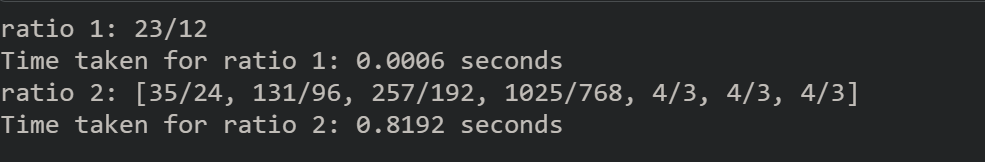
\includegraphics[scale=0.5]{ex1_1.png} \\
For ratio3, note that the output list below means 
the parameter $k$ runs from 1 up to $n$.
We get \\
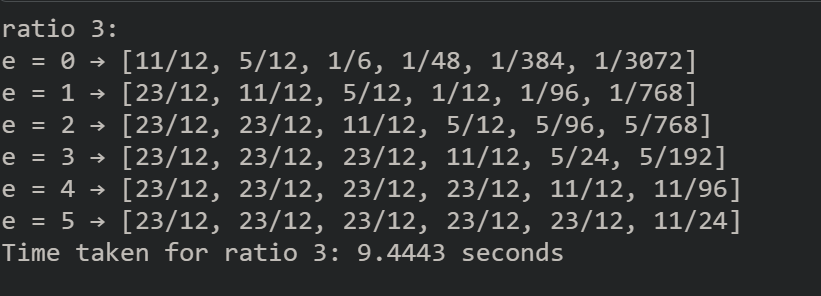
\includegraphics[scale=0.5]{ex1_2.png}

\item $p=2, n=7, M' = \begin{pmatrix}
1 & 0 \\ 0 & 1
\end{pmatrix}.$ \\
For ratio1 and ratio2 with $kmax = 8, \dots, 14$, we get \\
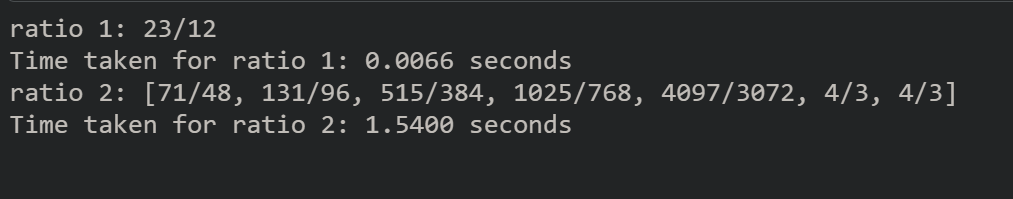
\includegraphics[scale=0.5]{ex2_1.png} \\
For ratio3, we get \\
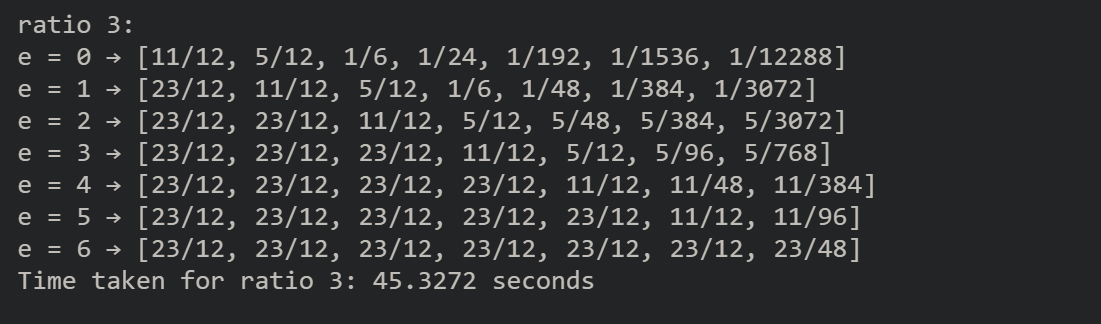
\includegraphics[scale=0.5]{ex2_2.png}

\item $p=2, n=8, M' = \begin{pmatrix}
1 & 0 \\ 0 & 1
\end{pmatrix}.$ \\
For ratio1 and ratio2 with $kmax = 9, \dots, 16$, we get \\
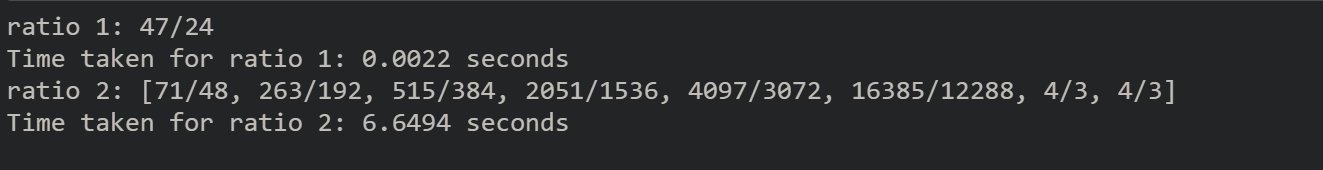
\includegraphics[scale=0.5]{ex3_1.png} \\
For ratio3, we get \\
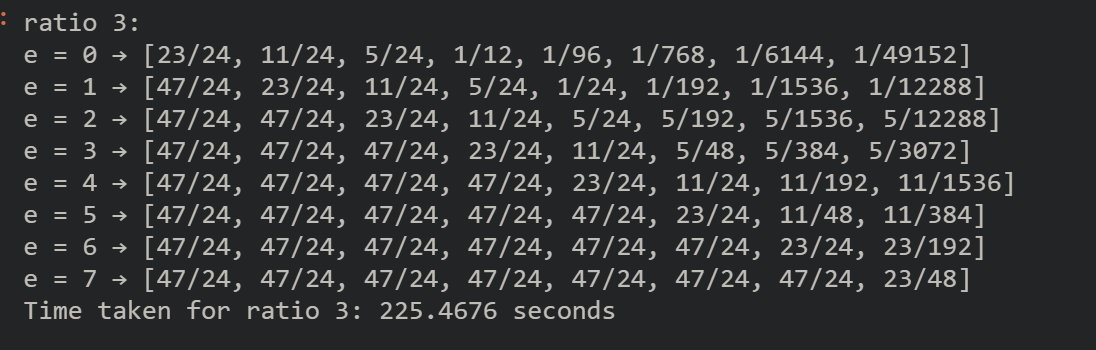
\includegraphics[scale=0.5]{ex3_2.png}

\item $p=2, n=8, M' = \begin{pmatrix}
3 & 0 \\ 0 & 7
\end{pmatrix}.$ \\
For ratio1 and ratio2 with $kmax = 9, \dots, 13$, we get \\
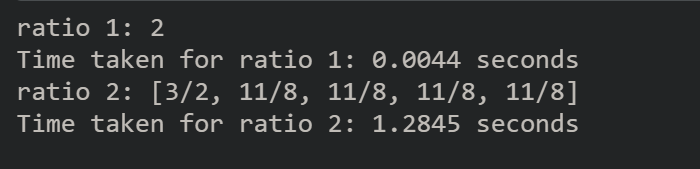
\includegraphics[scale=0.5]{ex9_1.png} \\
For ratio3, we get \\
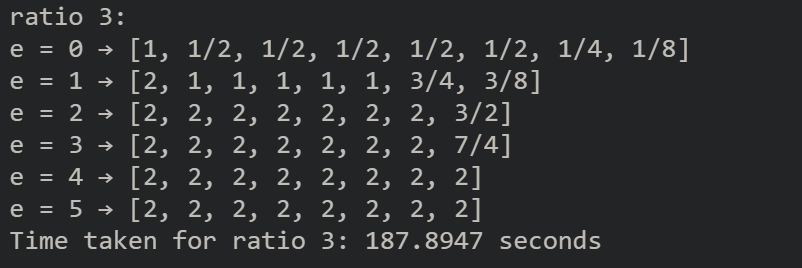
\includegraphics[scale=0.5]{ex9_2.png}

\item $p=3, n=5, M' = \begin{pmatrix}
1 & 0 \\ 0 & 4
\end{pmatrix}.$ \\
For ratio1 and ratio2 with $kmax = 6, \dots, 9$, we get \\
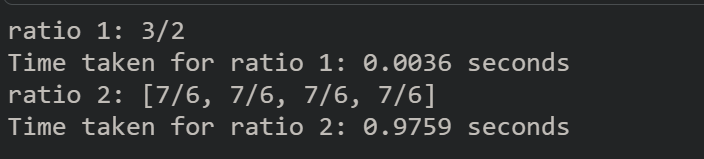
\includegraphics[scale=0.5]{ex4_1.png} \\
For ratio3, we get \\
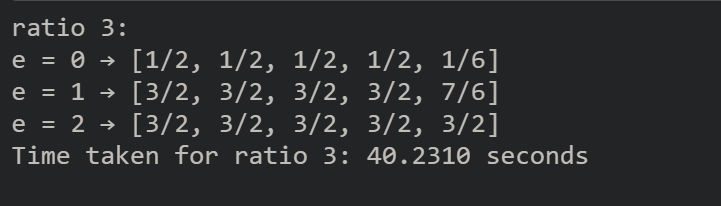
\includegraphics[scale=0.5]{ex4_2.png}

\item $p=3, n=6, M' = \begin{pmatrix}
1 & 0 \\ 0 & 10
\end{pmatrix}.$ \\
For ratio1 and ratio2 with $kmax = 7, \dots, 10$, we get \\
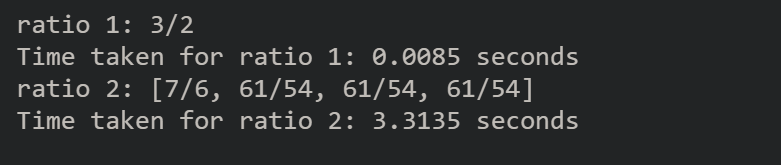
\includegraphics[scale=0.5]{ex5_1.png} \\
For ratio3, we get \\
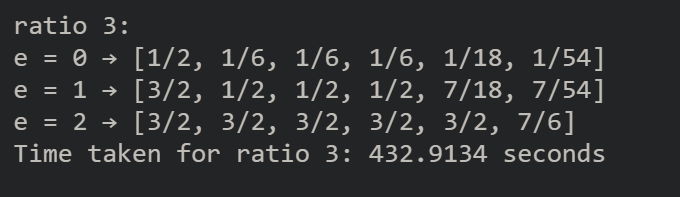
\includegraphics[scale=0.5]{ex5_2.png}

\item $p=3, n=6, M' = \begin{pmatrix}
1 & 0 \\ 0 & 28
\end{pmatrix}.$ \\
For ratio1 and ratio2 with $kmax = 7, \dots, 10$, we get \\
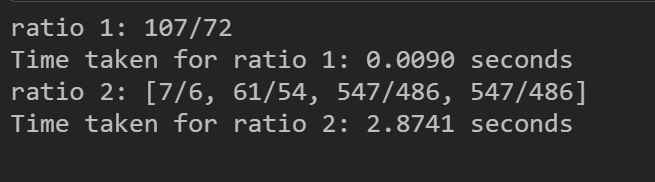
\includegraphics[scale=0.5]{ex6_1.png} \\
For ratio3, we get \\
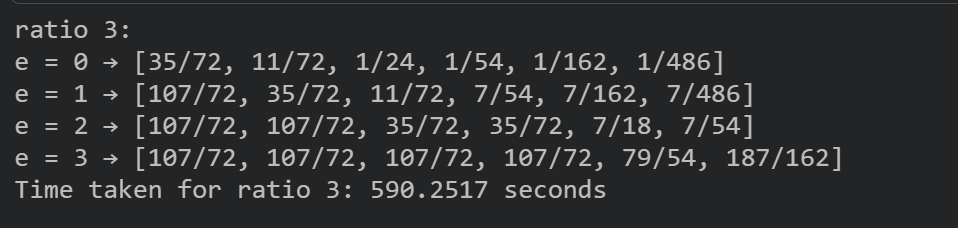
\includegraphics[scale=0.5]{ex6_2.png}

\item $p=5, n=4, M' = \begin{pmatrix}
2 & 0 \\ 0 & 3
\end{pmatrix}.$ \\
For ratio1 and ratio2 with $kmax = 5, \dots, 10$, we get \\
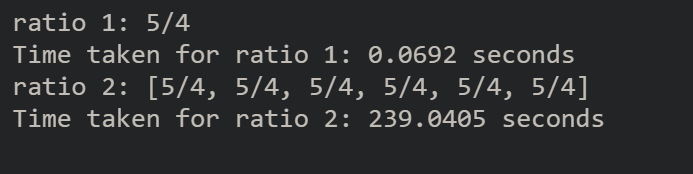
\includegraphics[scale=0.5]{ex7_1.png} \\
For ratio3, we get \\
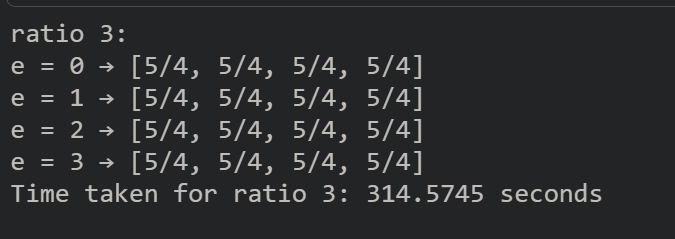
\includegraphics[scale=0.5]{ex7_2.png}

\item $p=5, n=4, M' = \begin{pmatrix}
1 & 0 \\ 0 & 6
\end{pmatrix}.$ \\
For ratio1 and ratio2 with $kmax = 5, \dots, 10$, we get \\
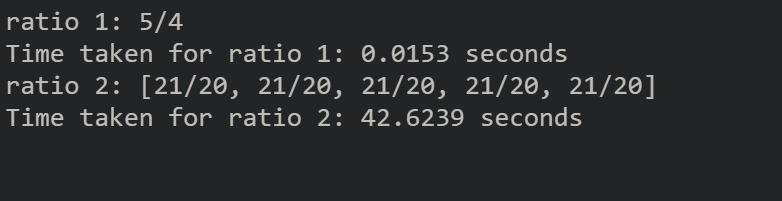
\includegraphics[scale=0.5]{ex8_1.png} \\
For ratio3, we get \\
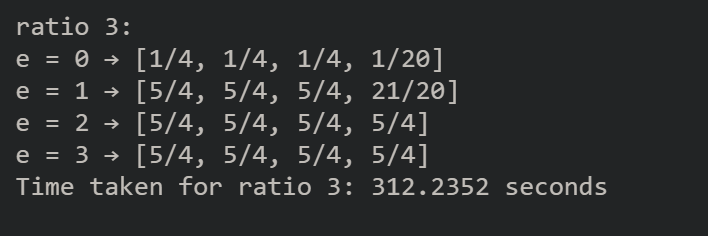
\includegraphics[scale=0.5]{ex8_2.png}

\end{enumerate}

%% Anything that comes after the ``\end{document}'' will be ignored.
\end{document}
